\documentclass[tikz,border=10pt]{standalone}
% Scale s = 0.02122 (from STYLE METRICS), y axis flipped, origin at ink-bbox centre (226.5, 202.5) px
\begin{document}
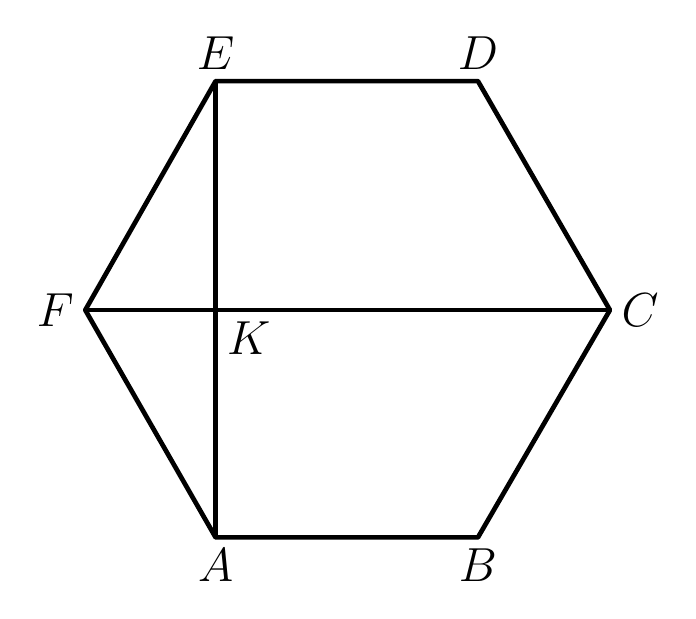
\begin{tikzpicture}[line join=round, line width=1.7pt]
  % Vertices (converted from pixels)
  \coordinate (F) at (-3.342,0.011);
  \coordinate (E) at (-1.687,2.918);
  \coordinate (D) at (1.645,2.918);
  \coordinate (C) at (3.321,0.011);
  \coordinate (B) at (1.645,-2.876);
  \coordinate (A) at (-1.687,-2.876);
  \coordinate (K) at (-1.687,0.011);

  % Hexagon sides
  \draw (F) -- (E) -- (D) -- (C) -- (B) -- (A) -- cycle;
  % Interior segments through K
  \draw (F) -- (C);
  \draw (E) -- (A);

  % Labels
  \node[above, font=\fontsize{17}{20.4}\selectfont] at (E) {$E$};
  \node[above, font=\fontsize{17}{20.4}\selectfont] at (D) {$D$};
  \node[right, font=\fontsize{17}{20.4}\selectfont] at (C) {$C$};
  \node[left, font=\fontsize{17}{20.4}\selectfont] at (F) {$F$};
  % K label: lower-right of the intersection (north west anchor at K)
  \node[anchor=north west, font=\fontsize{17}{20.4}\selectfont] at (K) {$K$};
  \node[below, font=\fontsize{17}{20.4}\selectfont] at (A) {$A$};
  \node[below, font=\fontsize{17}{20.4}\selectfont] at (B) {$B$};
\end{tikzpicture}
\end{document}